\chapter{Simultaneous Game}
Simultaneous games have randomness involved in it because of the action of second player is unknown. It is also finite horizon game which means agent can achieve rewards over finite steps. Since the work done in this field is on  Goeff-spiel so we have created a simultaneous environment of cricket and did the experiment on the top it with the algorithm of learning through self-play.

\section{Construction }
The game environment is set up in the following ways: 


We have two network one is bowler network and other is batsman network. The bowler network tries to choose which  bowler will bowl the  over. We have 5 bowlers which have some gradation in terms of bowling strength. Example first bowler will give less runs and more wicket whereas second bowler will give more runs than first bowler and can take less wickets and similarly strength decreases with third, fourth and fifth bowler.

The other network is batting network. There is batsman gradation similar to bowlers team. So first batsman can hit higher score than the second batsman. It tries to pick shots between 0, 1, 2, 4, 6 runs. The batting network will predict the probability of picking that shots such that it maximizes the runs score by the time. 

Moreover for simplicity the shot is fixed for a over game. Also  a simulator is defined which take batsman, bowler, shots and then predict the runs and wicket in that over. The implementation of it can be found here \url{https://github.com/vishalkumarchaudhary/connect4/tree/cricket-single-network}

State comprises of 8-tuples i.e. (total runs , wicket in hand, overs left, overs left for bowler1, overs left for bowler2, overs left for bowler3, overs left for bowler4, overs left for bowler5).
This state information is passed to both network for the corresponding predictions.


\section{Why not KL-UCB and Thompson bound?}
For the KL-UCB, the reward should be 0 or 1. Since the reward in cricket game is real number realization,so  we cannot use this kind of reward into this framework. For the same reason the Thompson bound requires the reward to be between [0,1] so for the same reason that rewards in cricket cannot be bounded or if bounded by taking the highest possible run and scaling it down then the reward we get by actually playing is concentrated to lower half and hence it would take a lot of time to learn for the agent.


\section{Observations}
\begin{enumerate}
    \item In sequential game, when both network are separated, then also the agent is able to learn but in the case of this game, the agent does not learn things at all. This is observed by looking the loss function of both network which was increasing or being horizontally straight line in every experiments for even 100 epochs.
    \item When the network was combined in such a way that first 2 layer was same for both network then the next 2 layer were different for both. So the network looks like two head outputs and single input layer network.
    
\end{enumerate}

\section{Results}
With the second model being both neural network combined, the bowling and batting network started learning. 
\subsection{Neural Network Loss}
\begin{figure}
 	[!htb]\centering
    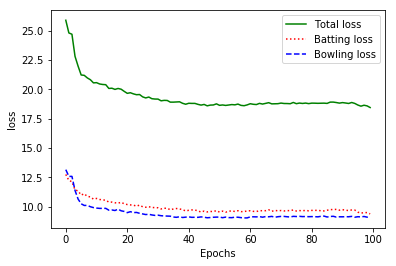
\includegraphics[width=6in]{images/ucb_cricket.png}
    \caption{Cricket Loss function during the training of Neural Network with $UCB1$ confidence bound}
  \label{fig:phase}
  \end{figure}
 
By observing above, we can say that the network is learning things of the simultaneous cricket game. Since the learning curve is horizontally straight at $100^{th}$ epochs, it means that the neural network is not finding the loss function decreasing. It also implies that the network either has learned things and not able to learn further because of randomness involved in the problem. 
\subsection{Network predictions}
Investigating further inside the neural network prediction because we know the bowling network strategy because of gradation in bowling players.
State is  (total runs ,  wicket in hand,  overs left,  overs left for bowler1,  overs  left  for  bowler2,  overs  left  for  bowler3,  overs  left  for  bowler4,  overs  left for  bowler5)
Predictions of bowling network:


\begin{table}[h!]
\center
\begin{tabular}{ |c||c|}

 \hline
 States    &  predictions[bowler 1 to 5]\\
 \hline
[239,   6,    15,   3,   3,   3,   3,   3] &[ \textbf{1.000e+00, 0.000e+00, 0.000e+00, 0.000e+00}] \\
\hline
[61,  8,  5,  1,  1,  1,  1,  1] & [\textbf{9.936e-01, 2.24e-04, 3.1020e-05,2.686e-04,3.752e-04}] \\
 \hline
 [457,   3,  10,   2,   2,   2,   2,   2] & [\textbf{1.000e+00, 0.000e+00, 0.000e+00, 0.000e+00, 7.410315e-29}]\\
\hline
[212, 5, 14, 0, 2, 12, 2, 0] & [0.9312 ,\textbf{ 0.18058, 0.9999 , 0.9999 , 0.4244}] \\
\hline
[411, 5, 4, 0, 0, 4, 2, 0] & [0.9985044 , 0.01386932,\textbf{ 1.        , 1.        , 0.20514968}]\\
\hline 
[411, 5, 2, 0, 0, 0, 1, 1] &  [0.99880195, 0.01228645, 0.3        , \textbf{1.        , 0.19677433}]\\ 
\hline
 
\end{tabular}
\caption{Blower network Prediction}
\label{table:1}
\end{table}

\subsection{Conclusion}
The bowling network is trained for 30 overs in the above tables. After masking invalid actions for the output of the network, we can see desired output which has maximum for choosing that bowler with maximum strength. During investigation it is also observed that sometime it tries to predict the wrong bowler with maximum number but for only one bowler. Moreover this is not the probability though it can be mapped by dividing with sum of all and choosing the maximum number.
